\newcommand{\tab}{\hspace*{2em}}
\chapter{Literature Review} 

\section{Power Measurement}
{
Most current sensors can measure current in two directions.  this means is that if we sample fast enough and long enough,  we sure to find the peak in one direction and the peak in another direction. With both peaks known, it is a matter of knowing the shape of the waveform to calculate the current. In the case of line or mains power, we know that waveform to be a Sine wave. Hence the expression of AC current  will be in a value known as RMS. 

\begin{figure}[H]
	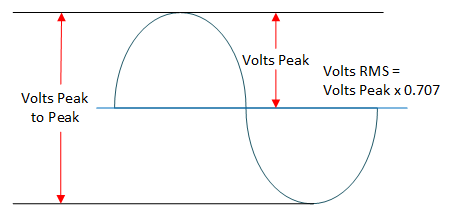
\includegraphics[scale=1]{vrms} % first figure itself
	\caption{Measurement of Vrms}
	\label{blck}
\end{figure}

Conversion for a sine wave with a zero volt offset (like that in mains or line power) is performed as follows:

\begin{enumerate}
	\item Find the peak to peak voltage  ( Volts Peak to Peak )
	\item Divide the peak to peak voltage by two to get peak voltage (Volts Peak)
	\item Multiply the peak voltage by 0.707 to yield rms volts (Volts RMS)
\end{enumerate}

Having Calculated RMS voltage,  is simply a matter of multiplying by the scale factor of the particular current sensor to yield the RMS value of the current being measured which can then be multiplied by the AC Voltage value in order to give the value of the Total Power Drawn.

\begin{equation}
I_r_m_s = \frac{V_p_p \times 0.707 \times Scale Factor}{2} 
\end{equation}

\begin{equation}
P = I_r_m_s \times 230
\end{equation}

}



\section{Disaggregation Algorithms}
Most NLIM systems provide implementations of two common benchmark
disaggregation algorithms: Steady State Analysis and Combinatorial Optimisation(CO).

\subsection{Steady State Analysis}
The NILM methods based on steady-state analysis make use of steady-state features that are derived
under the steady-state operation of the appliances. Real power (P) and Reactive power (Q) are two of the
most commonly used steady state signatures in NILM  for tracking On/Off operation of appliances.
The real power is the amount of energy consumed by an appliance during its operation. If the load is
purely resistive then the current and voltage waveforms will always be in phase and there will be no
reactive energy. For a purely reactive load the phase shift will be 90 degrees, and there will be no transfer of real
power. On the other hand, due to inductive and capacitive elements of the load, there is always a phase
shift between current and voltage waveforms that generates or consumes a reactive power respectively.

\begin{figure}[H]
	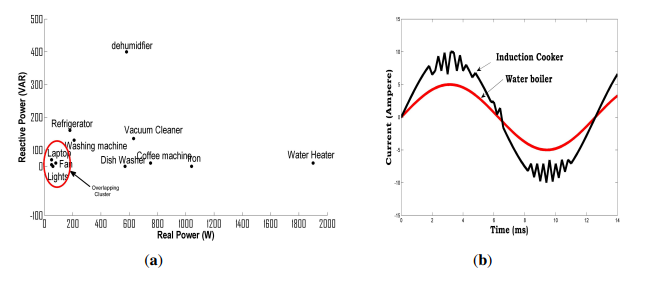
\includegraphics[scale=1]{steadystate} % first figure itself
	\caption{Load Distribution in PQ Plane and Current draw of Linear vs Non Linear Loads}
	\label{blck}
\end{figure}

Researchers have tried to disaggregate load using real power as a single feature and found
out that high-power appliances with distinctive power draw characteristics such as electrical heaters and
water pumps can be easily identified from the aggregated measurements. However this method does
not take into account appliances with similar power draw characteristics. In addition, simultaneous state
transitions of appliances leads to erroneous results. In order to address some of these issues, high power appliances can easily be differentiated
by analyzing the step changes in real and reactive power features.

\subsection{Combinational Optimization(CO)}

Combinational Optimization finds the optimal combination of appliance states, which minimizes the difference between the sum of the predicted appliance power and the observed aggregate power, subject to a set of appliance models. Since each time slice is considered as a separate optimisation problem, each time slice is assumed to be independent.
The complexity of disaggregation for T time slices is: 

\begin{equation}
N_C_o_m_b_i_n_a_t_i_o_n_s = K ^ N
\end{equation}

where N is the number of appliances and
K is the number of appliance states.

Since the complexity of CO is exponential in the number of appliances, the approach is only computationally tractable for a small number of modelled appliances. The error can be minimized by choosing the combination whose calculated power draw is the closest to the measured power drawn.

\subsection{K Nearest Neighbours(KNN)}
In pattern recognition, the k-nearest neighbors algorithm (k-NN) is a non-parametric method used for classification and regression. In both cases, the input consists of the k closest training examples in the feature space. The output depends on whether k-NN is used for classification or regression:

In k-NN classification, the output is a class membership. An object is classified by a majority vote of its neighbors, with the object being assigned to the class most common among its k nearest neighbors (k is a positive integer, typically small). If k = 1, then the object is simply assigned to the class of that single nearest neighbor.
In k-NN regression, the output is the property value for the object. This value is the average of the values of its k nearest neighbors.
k-NN is a type of instance-based learning, or lazy learning, where the function is only approximated locally and all computation is deferred until classification. The k-NN algorithm is among the simplest of all machine learning algorithms.

Both for classification and regression, it can be useful to assign weight to the contributions of the neighbors, so that the nearer neighbors contribute more to the average than the more distant ones. For example, a common weighting scheme consists in giving each neighbor a weight of 1/d, where d is the distance to the neighbor.

The neighbors are taken from a set of objects for which the class (for k-NN classification) or the object property value (for k-NN regression) is known. This can be thought of as the training set for the algorithm, though no explicit training step is required.

A peculiarity of the k-NN algorithm is that it is sensitive to the local structure of the data.[citation needed] The algorithm is not to be confused with k-means, another popular machine learning technique. 
 Following example would help us to understand better :
 The test sample (green circle) should be classified either to the first class of blue squares or to the second class of red triangles. If k = 3 (solid line circle) it is assigned to the second class because there are 2 triangles and only 1 square inside the inner circle. If k = 5 (dashed line circle) it is assigned to the first class (3 squares vs. 2 triangles inside the outer circle). 
\begin{figure}
    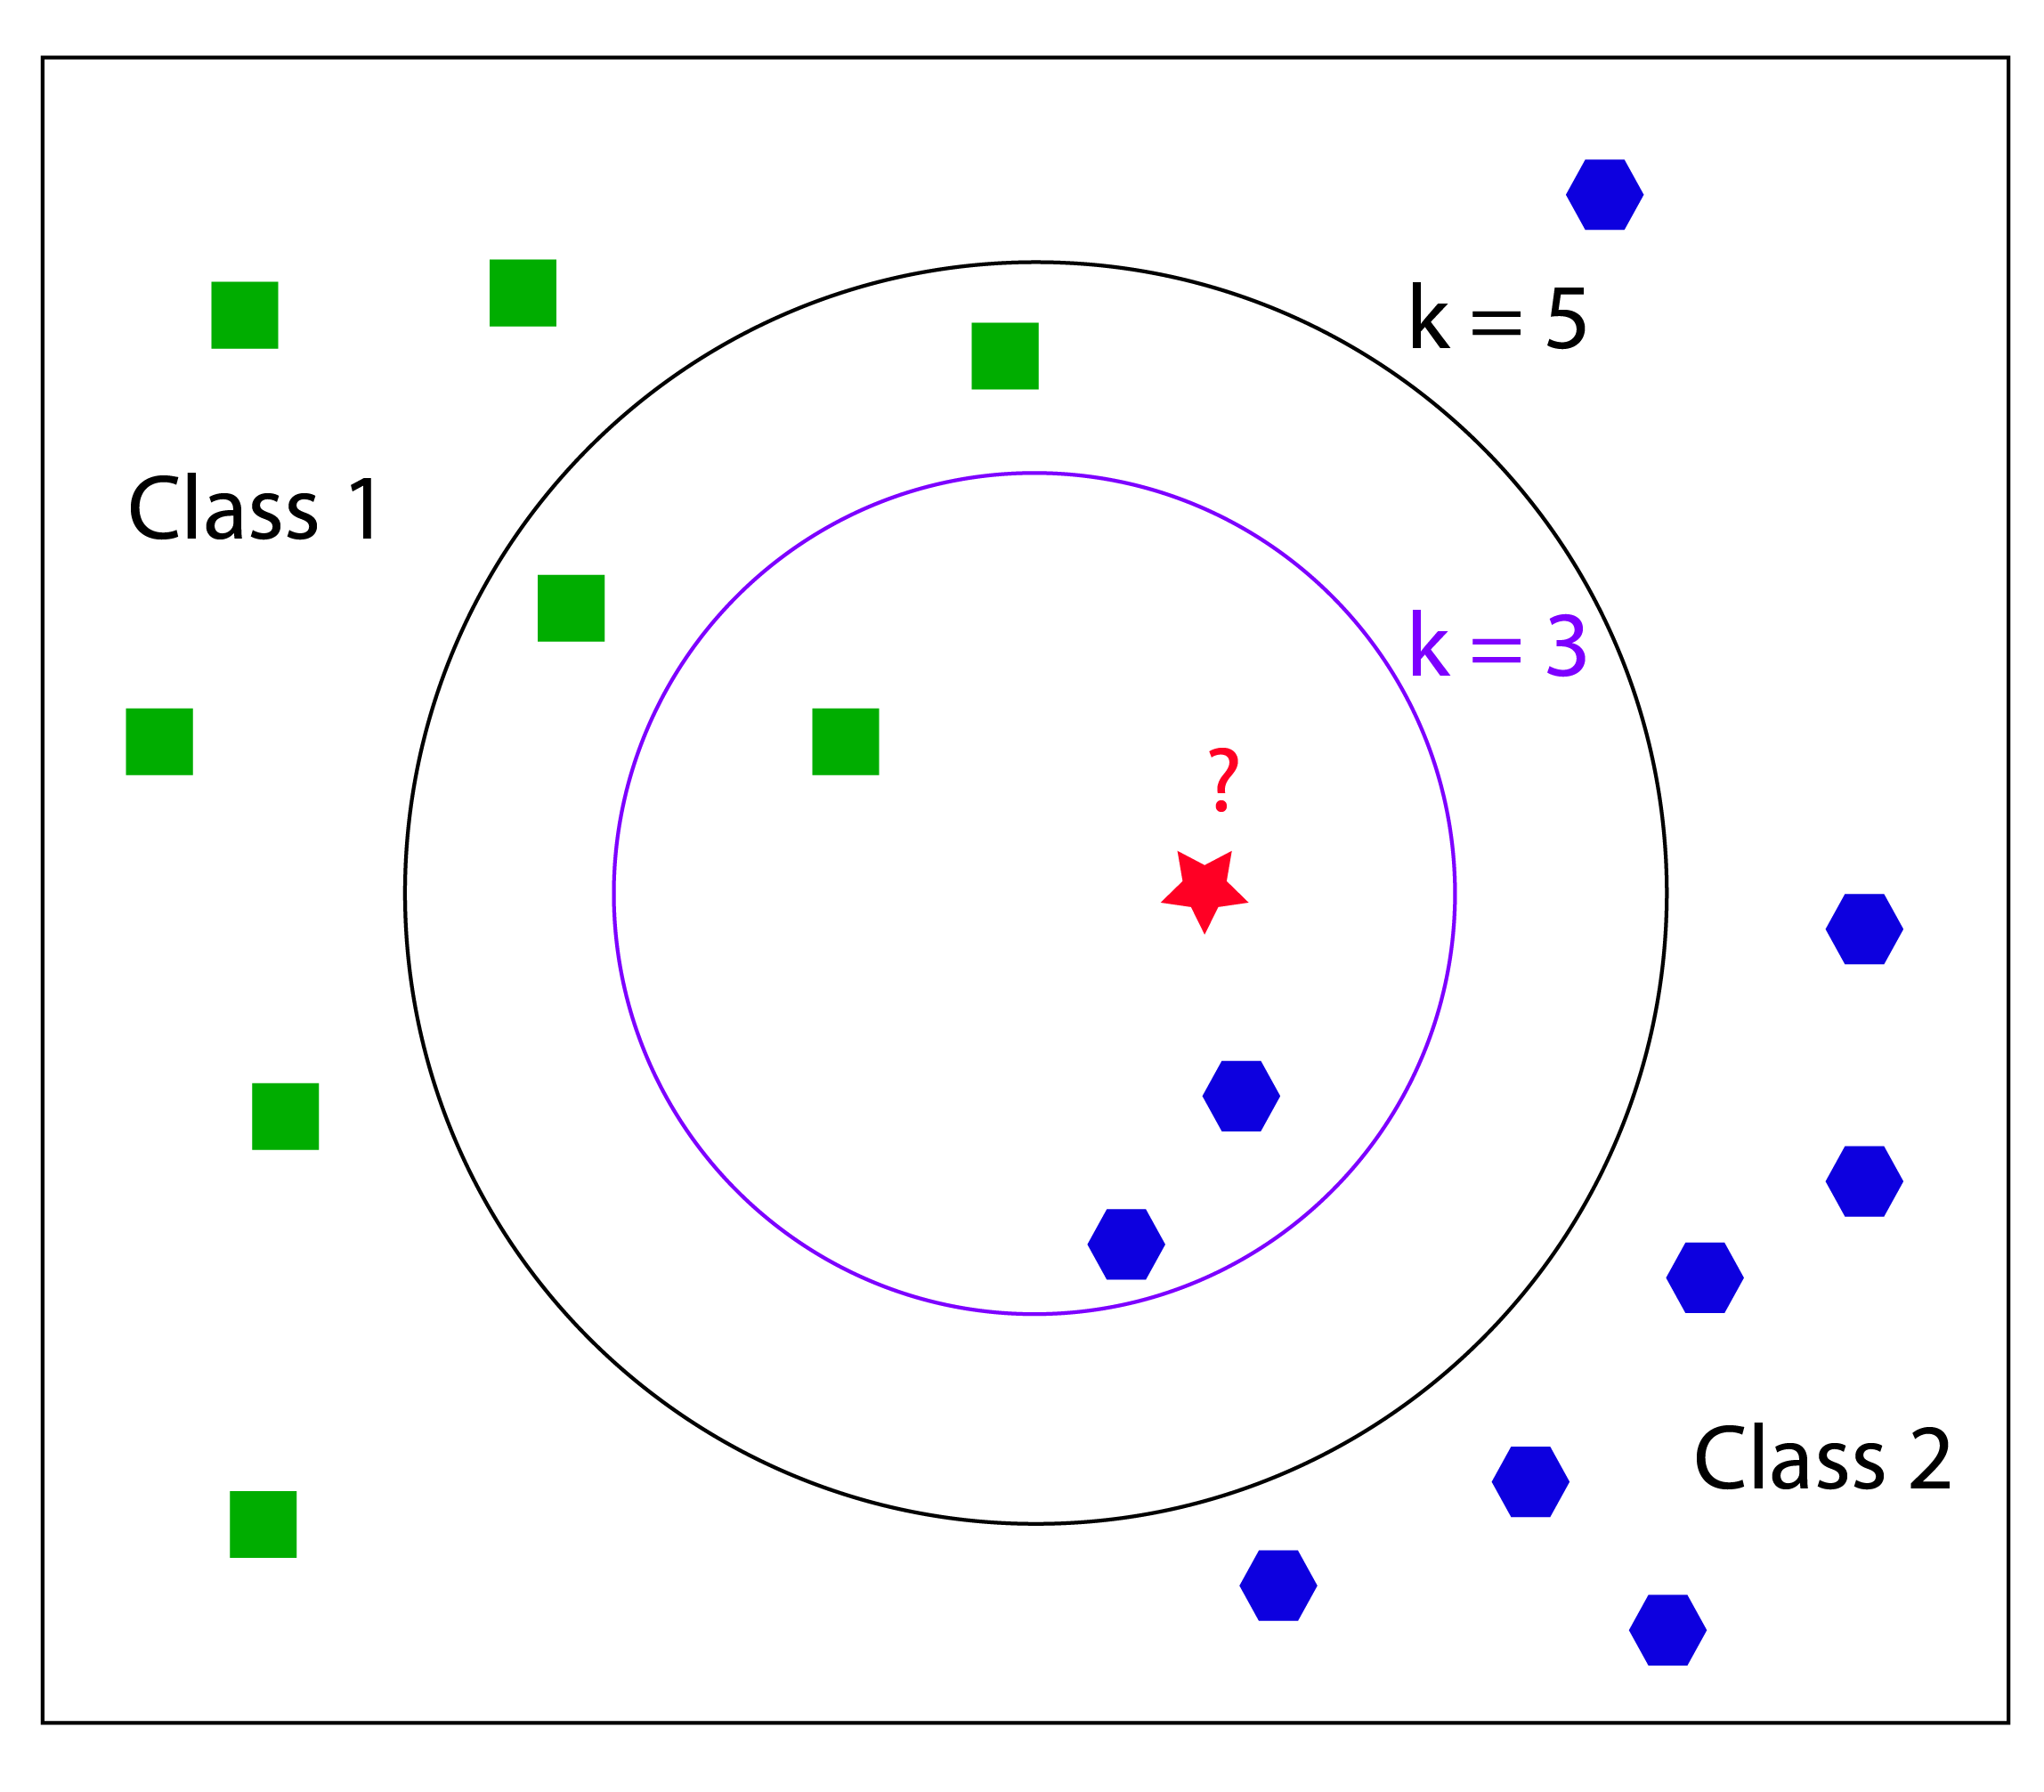
\includegraphics[width=0.9\textwidth]{images/knn.png}
    \caption{K Nearest Neighbour}
    \label{fig:my_label}
\end{figure}

\section{Public Datasets}

Apart from a common evaluation metric there is also a lack of reference dataset on which the
performance of algorithm can be compared. It is quite obvious that the output of the load disaggregation
algorithm is dependent on the source data, which often varies either due to difference in the number
and type of appliances used in the experiment or due to the hardware used to extract the load signatures. In order to draw meaningful performance comparison of various NILM techniques,
the availability of common datasets is critical. Motivated by this, recently the Reference Energy Disaggregation Data Set (REDD) and the Building-Level fUlly labeled Electricity Disaggregation dataset (BLUED) have been made publicly available in order to facilitate the researchers in the development and evaluation of new load disaggregation algorithms. The datasets contain high-frequency and low-frequency household power measurements primarily for the evaluation of steady-state as well as transient state NILM methods.

\subsection{Reference Energy Disaggregation Dataset (REDD)}
The data contains power consumption from real
homes, for the whole house as well as for each individual circuit in
the house (labeled by the main type of appliance on that circuit).
The data is intended for use in developing disaggregation methods, which
can predict, from only the whole-home signal, which devices are being
used. The REDD data set contains two main types of home electricity data:
high-frequency current/voltage waveform data of the two power mains
(as well as the voltage signal for a single phase), and
lower-frequency power data including the mains and individual,
labeled circuits in the house. 

\subsection{Building-Level fUlly labeled Electricity Disaggregation (BLUED) Dataset}
The BLUED dataset consists of voltage and current measurements for a single family residence in the United States, sampled at 12 kHz for a whole week. Every state transition of each appliance in the home during this time was labeled and time-stamped, providing the necessary ground truth for the evaluation of event-based algorithms. 















 
 
 
 
 
 
 
 
 
 
 

 
 
 
 
 
 
 

